\newpage\thispagestyle{empty}
  \begin{tabular}{p{6cm} p{8cm}}
      \begin{minipage}{7cm}
      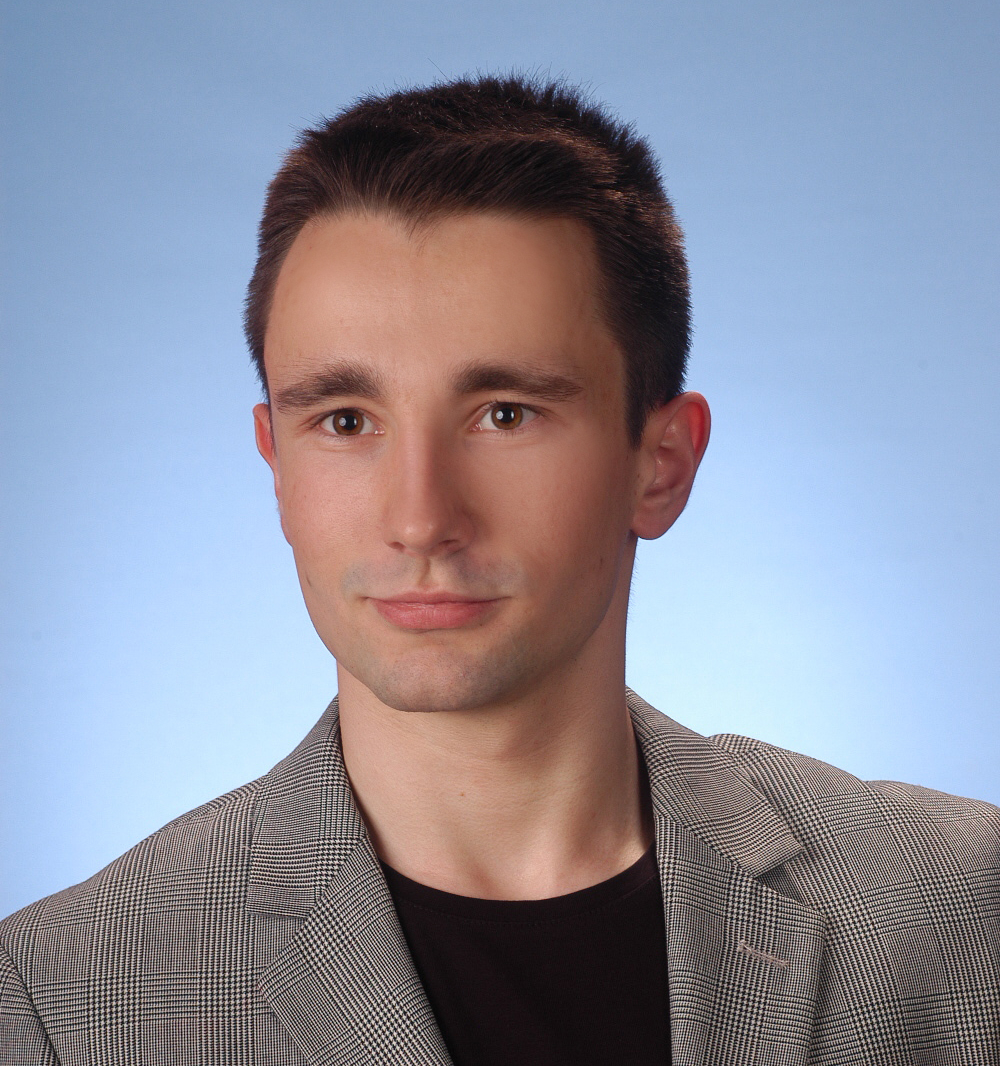
\includegraphics[height=6cm, keepaspectratio]{img/author-photo.jpg}
      \end{minipage}
      &
      \begin{minipage}{8cm}
      Kierunek: \\[\smallskipamount]
      {\large Informatyka}\\[0.2cm]
      Specjalność: \\[\smallskipamount]
      {\large Inżynieria Systemów Informacyjnych}\\[0.2cm]
      Data urodzenia: \\[\smallskipamount]
      {\large 13 maja 1991r.}\\[0.2cm]
      Data rozpoczęcia studiów: \\[\smallskipamount]
      {\large 1 października 2014r.}
      \end{minipage}
  \end{tabular}
  \vspace*{1\baselineskip}
  \begin{center}
  {\large\bfseries Życiorys}\par\bigskip
  \end{center}
  Urodziłem się 13 maja 1991 roku. W 2010 roku ukończyłem II Liceum Ogólnokształcące
  im. Romualda Traugutta w Częstochowie. W 2014 roku uzyskałem tytuł inżyniera informatyki na~Wydziale Elektroniki
  i~Technik Informacyjnych Politechniki Warszawskiej (specjalność: Inżynieria Systemów Informacyjnych).
  W~tym~samym roku rozpocząłem studia magisterskie na~tym~samym wydziale, kierunku i~specjalności.
  Podczas studiów drugiego stopnia odbyłem roczny staż w~Europejskiej Organizacji Badań Jądrowych (CERN) w~Genewie.
  W~ramach jednego z~eksperymentów zajmowałem się~projektowaniem i~implementacją sztucznych sieci neuronowych.

  \indent

  \hfill\parbox{15em}{{\small\dotfill}\\[-.3ex]
  \centerline{\footnotesize podpis studenta}}\par
  \vspace{2\baselineskip}
  \begin{center}
  {\large\bfseries Egzamin dyplomowy} \par\bigskip\bigskip
  \end{center}
  \par\noindent
  Złożył egzamin dyplomowy w dn. \dotfill 2017r
  \par\noindent
  Z wynikiem \dotfill
  \par\noindent
  Ogólny wynik studiów \dotfill
  \par\noindent
  Dodatkowe wnioski i uwagi Komisji \dotfill
  \par\noindent
  \dotfill